\documentclass{article}


% if you need to pass options to natbib, use, e.g.:
%     \PassOptionsToPackage{numbers, compress}{natbib}
% before loading neurips_2024


% ready for submission
\usepackage{neurips_2024}


% to compile a preprint version, e.g., for submission to arXiv, add add the
% [preprint] option:
%     \usepackage[preprint]{neurips_2024}


% to compile a camera-ready version, add the [final] option, e.g.:
%     \usepackage[final]{neurips_2024}


% to avoid loading the natbib package, add option nonatbib:
%    \usepackage[nonatbib]{neurips_2024}


\usepackage[utf8]{inputenc} % allow utf-8 input
\usepackage[T1]{fontenc}    % use 8-bit T1 fonts
\usepackage{hyperref}       % hyperlinks
\usepackage{url}            % simple URL typesetting
\usepackage{booktabs}       % professional-quality tables
\usepackage{amsfonts}       % blackboard math symbols
\usepackage{nicefrac}       % compact symbols for 1/2, etc.
\usepackage{microtype}      % microtypography
\usepackage{xcolor}         % colors
\usepackage{graphicx}
\usepackage{amsmath}
\usepackage{amsthm}
\usepackage{float}
\usepackage{bm}

\newtheorem{theorem}{Proposition}
\newtheorem{corollary}{Corollary}[theorem]

\title{Contrastive Optimization -- Preliminaries}


% The \author macro works with any number of authors. There are two commands
% used to separate the names and addresses of multiple authors: \And and \AND.
%
% Using \And between authors leaves it to LaTeX to determine where to break the
% lines. Using \AND forces a line break at that point. So, if LaTeX puts 3 of 4
% authors names on the first line, and the last on the second line, try using
% \AND instead of \And before the third author name.


\author{%
  David S.~Hippocampus\thanks{Use footnote for providing further information
    about author (webpage, alternative address)---\emph{not} for acknowledging
    funding agencies.} \\
  Department of Computer Science\\
  Cranberry-Lemon University\\
  Pittsburgh, PA 15213 \\
  \texttt{hippo@cs.cranberry-lemon.edu} \\
  % examples of more authors
  % \And
  % Coauthor \\
  % Affiliation \\
  % Address \\
  % \texttt{email} \\
  % \AND
  % Coauthor \\
  % Affiliation \\
  % Address \\
  % \texttt{email} \\
  % \And
  % Coauthor \\
  % Affiliation \\
  % Address \\
  % \texttt{email} \\
  % \And
  % Coauthor \\
  % Affiliation \\
  % Address \\
  % \texttt{email} \\
}


\begin{document}


\maketitle


% \begin{abstract}
%   The abstract paragraph should be indented \nicefrac{1}{2}~inch (3~picas) on
%   both the left- and right-hand margins. Use 10~point type, with a vertical
%   spacing (leading) of 11~points.  The word \textbf{Abstract} must be centered,
%   bold, and in point size 12. Two line spaces precede the abstract. The abstract
%   must be limited to one paragraph.
% \end{abstract}


\section{Background \& Motivation}

The standard optimization pipeline for image classification predominantly consists of using a CNN-backbone with a fully-connected layer pointing to the classification targets.

This setup is vulnerable to spurious correlation caused by features like a common background, causing the model to learn `tricks', bypassing actually learning the target features. A simple example is illustrated in the second paragraph of the introduction in \cite{arjovsky2020invariantriskminimization}.

A popular post-hoc technique -- Class Activation Mappings \citep{zhou2016learning} -- helps diagnose this by generating a heatmap that visualizes the regions of the image used by the model to generate the prediction. Further research uncovered that the interpretation used by CAMs, and it's derivative GradCAMs were unfaithful as a consequence of the averaging step.

HiResCAM \citep{draelos2020use} is a variant of GradCAM \citep{selvaraju2017grad} that demonstrates that their visualization \textbf{provably recovers the input-dependent abnormality score} from the final classification. Therefore, there is a guarantee associated with the faithfulness of the visualization.

This approach derives an interpretable training objective using HiResCAMs, which replaces and outperforms cross-entropy loss to build an intrinsically interpretable, performant model.

\section{Methodology}

The experimental setup is a CNN-backbone (here, ResNet-50) with a single fully connected softmax-activated layer for classification. The backbone outputs feature maps $\bm{A} \in \mathbb{R}^{F \times D_1 \times D_2}$, which is flattened to $\bm{A}_F \in \mathbb{R}^{FD_1D_2 \times 1}$ and fed to the linear layer with $\bm{w}_c \in \mathbb{R}^{1 \times FD_1D_2}$. The logits obtained in $\mathbb{R}^{c}$, where $c$ is the total number of classes is then passed through softmax to generate the final probabilities.

\subsection{Observation: HiResCAMs Explain Class Score, Not Class Probabilites}

Per \cite{draelos2020use}, a HiResCAM is defined as follows:
\begin{gather}
	\tilde{\mathcal{\bm{A}}}_c^{\text{HiResCAM}} = \sum^F_{f=1} \frac{\partial s_c}{\partial \bm{A}^f} \odot \bm{A}^f
\end{gather}

Where $s_c$ denotes the logit for a single class. $\tilde{\mathcal{\bm{A}}}_c^{\text{HiResCAM}}$ generates a class-specific CAM. For the CAM architecture, \cite{draelos2020use} (section 3.6.2) shows that:
\begin{gather}
	\sum^{D_1,D_2}_{i,j} \tilde{\mathcal{\bm{A}}}_{c,i,j}^{\text{HiResCAM}} = \frac{\bm{w}_c \bm{A}_F}{D_1 D_2} \\
	s_c = \frac{\bm{w}_c \bm{A}_F}{D_1 D_2} + b_c = \sum^{D_1,D_2}_{i,j} \tilde{\mathcal{\bm{A}}}_{c,i,j}^{\text{HiResCAM}} + b_c
\end{gather}
Therefore, we can recreate the entire input-dependent part of the score using HiResCAMs. Doing this for each class $c$, we obtain the bias-removed logit vector $\in \mathbb{R}^{c}$.

The standard interpretation of this result uses the obtained activation maps as explanations for the prediction. Popular practice is to follow this up by ReLU and normalization \citep{draelos2020use}. However, since softmax is computed over the logit vector, this interpretation is flawed.

We can consider the backbone as a kernel that attempts to linearly separate the correct class, with the softmax-activated final layer just being logistic regression over the final feature map.

In this setup, each class has it's own set of weights that feedforwards independently, but trains collaboratively. It assigns a score for it's specific value, which is independent since one set of weights does not affect the other over a forward pass. A consequence of performing softmax over the final logits is that the normalization steps renders only the difference between each score $s_c$ relevant for the final prediction probability.

\begin{theorem}
	Individual class probabilites $\sigma_c(\bm{s})$ depend on the difference(s) between class logits.
\end{theorem}
\begin{proof} Individual class probabilities for logit vector $\bm{s}$ are defined as:
	\begin{gather}
		\sigma_c(\bm{s}) = \frac{e^{s_c}}{\sum_i e^{s_i}}
	\end{gather}
	We define our logit vector in terms of the elementwise difference to a target class $c$:
	\begin{gather}
		d = [s_i - s_c]_i \\
		\bm{s} = [s_c + d_i]_i
	\end{gather}
	Based on this definition, class probabilities can now be computed as:
	\begin{align}
		\sigma_c(\bm{s}) &= \frac{e^{s_c}}{\sum_i e^{s_c+d_i}} \\
				 &= \frac{e^{s_c}}{e^{s_c} \sum_i e^{d_i}} = \frac{1}{\sum_i e^{d_i}}
	\end{align}
	This recontextualizes softmax as a direct function of the differences of class logits.
\end{proof}
\begin{corollary} Since class probabilities depend on logit differences, the class probabilities are identitical for any two pairs of logit vectors with identical logit differences.
	\begin{gather}
		\frac{e^{s_c}}{\sum_i e^{s_i}} = \frac{e^{s_c+r}}{\sum_i e^{s_i+r}} \forall r \in \mathbb{R}
	\end{gather}
\end{corollary}
\begin{proof} Recontextualizing $\bm{s}$ per the previous proposition, we get:
	\begin{align}
		\frac{e^{s_c}}{\sum_i e^{s_c + d_i}} &= \frac{e^{s_c+r}}{\sum_i e^{s_c+d_i+r}} \\
		\frac{e^{s_c}}{e^{s_c}\sum_i e^{d_i}} &= \frac{e^{s_c+r}}{e^{s_c + r} \sum_i e^{d_i}} \\
		\frac{1}{\sum_i e^{d_i}} &= \frac{1}{\sum_i e^{d_i}}
	\end{align}
	Therefore, the absolute scale of a logit does not influence the final class probability.
\end{proof}

As an example, for logits $[1,2]$ and $[-2,-1]$, $\sigma([1,2]) = \sigma([-2,1]) = [0.2689, 0.7311]$. The prediction probabilities remain the same, despite different values for the same score $s_c$. Therefore, making inferences based on \textit{absolute score} results in a misrepresentation of the internal model state. Instead, the objective is to maximize the \textbf{difference between class logits}.

\subsection{Defining the Contrastive Optimization Objective}

We start by \textbf{comparing the contrast} of the activation maps with respect to one another. If for a single point $\bm{A}_{i,j}$, $\bm{w}_c > \bm{w}_{c'}$, that point is more likely to represent the object belonging to class $c$, even if the absolute value of $\bm{w}_{c'}$ is high. This information is lost during the flattening, which embeds positional invariance.

We therefore derive an optimization objective that attempts to maximize the contrast between the two activations maps. For the binary classification case, $(c, c')$ reflects that correct and incorrect class respectively.
\begin{gather}
	\max_{\theta} s_c - s_{c'} \equiv \max_{\theta} \sum^{D_1,D_2}_{i,j} \tilde{\mathcal{\bm{A}}}_{c,i,j}^{\text{HiResCAM}} + b_c - \sum^{D_1,D_2}_{i,j} \tilde{\mathcal{\bm{A}}}_{c',i,j}^{\text{HiResCAM}} - b_{c'}
\end{gather}
Ignoring the bias terms, our new optimization objective is:
\begin{gather}
	\max_{\theta} \tilde{\mathcal{\bm{A}}}^{\text{contrastive}} := \sum^{D_1,D_2}_{i,j} \tilde{\mathcal{\bm{A}}}_{c,i,j}^{\text{HiResCAM}} - \sum^{D_1,D_2}_{i,j} \tilde{\mathcal{\bm{A}}}_{c',i,j}^{\text{HiResCAM}}
\end{gather}
This is equivalent to the original ERM optimization objective, with the difference being the resultant values preserving spatial information as an activation map instead of flattening the feature map. If $\tilde{\mathcal{\bm{A}}}_{c}^{\text{HiResCAM}} - \tilde{\mathcal{\bm{A}}}_{c'}^{\text{HiResCAM}} > 0$, the classification is correct -- if not, the classification is incorrect. 

For the multiclass case, our setup now considers a set of classes $c$; $c_t$ is our target class, and $c_{t'}$ consists of a sampled non-target class. The definition for multiclass contrastive activation maps now results in a set of activation maps, defined as follows:
\begin{gather}
	\tilde{\mathcal{\bm{A}}}^{\text{contrastive}} := \{\tilde{\mathcal{\bm{A}}}_{c_t}^{\text{HiResCAM}} - \tilde{\mathcal{\bm{A}}}_{c_t'}^{\text{HiResCAM}}\}^{|c|-1}_{c_{t'} \in c - c_t}
\end{gather}
This is a generalization of the binary case, as the same formula applied to a binary classification challenge returns a set of contrastive maps containing a single element.

To ensure that the model accurately predicts the target class, each contrastive comparison should yield a positive result. Therefore, the multiclass optimization objective under this paradigm is as follows:
\begin{gather}
	\max_{\theta} \sum^{D_1,D_2}_{j,k}\tilde{\mathcal{\bm{A}}}_{i,j,k}^{\text{contrastive}}\ \forall i \in \mathbb{N}(|c| - 1)
\end{gather}

\subsection{Constraining Optimization to an Interpretable Basis}

As discussed in the previous section, the distinctive feature of the contrastive optimization objective over standard risk is that this preserves spatial information. We know at a pointwise level how each feature contributes to the final prediction.

We can use this to constrain the way optimization occurs -- namely, we only want the model to increase the likelihood of an object belonging to a certain class by actually looking at the features of the class, and not features of spurious correlation like the environment in which the object is present. The model through the process of training should learn to distinguish and subsequently ignore the background in determining the final prediction.

Segmentations maps describe the region over which the object is present. We can leverage this information to define a constrastive cost function as follows:
\begin{gather}
	\{(x, (h, y))\}^N \in \mathcal{D} \text{ where } h_{i,j} := \begin{cases}
		1 & \text{pixel contains subject} \\
		0 & \text{otherwise}
	\end{cases} \\
	\mathcal{\bm{A}}^{\text{background}}_{c,i,j} := \begin{cases}
		\tilde{\mathcal{\bm{A}}}^{\text{contrastive}}_{c,i,j} & h_{i,j} = 0 \\
		0 & \text{otherwise}
	\end{cases} \\
	\mathcal{\bm{A}}^{\text{foreground}}_{c,i,j} := \begin{cases}
		0 & h_{i,j} = 0 \\
		\tilde{\mathcal{\bm{A}}}^{\text{contrastive}}_{c,i,j} & \text{otherwise}
	\end{cases} \\
	D_{KL}(P || Q) := \frac{1}{|c|-1}\sum^{|c|-1}_c P \cdot \log \frac{P'}{Q_c} \text{ where } 
	P'_{i,j} := \begin{cases}
		1 & h_{i,j} \neq 0 \\
		P_{i,j} & \text{otherwise}
	\end{cases} \label{d_kl} \\
	\begin{split}
		\mathcal{\bm{J}}(\theta, \mathcal{D}) := &D_{KL}(\sigma_{\text{softmax}}(\lambda_1 \mathcal{\bm{A}}^{\text{contrastive}})\ ||\ \sigma_{\text{softmax}}(\lambda_2 h)) \\
		&+ \frac{\lambda_3}{D_1 D_2} ||\mathcal{\bm{A}}^{\text{background}}||^2_F \\
		&- \frac{1}{D_1 D_2} \sum^{|c|-1,D_1,D_2}_{c,i,j} \mathcal{\bm{A}}^{\text{foreground}}_{c,i,j}
	\end{split}
\end{gather}

The cost function has a threefold purpose:
\begin{enumerate}
	\item Minimize the divergence of the contrastive activation map to the segmentation map.
	\item Minimize the absolute value of the contrastive map where the segmentation map is the background.
	\item Maximize the value of the contrastive map where the segmentation map is the foreground.
\end{enumerate}

$D_{KL}$ is modified per (10), such that the likelihood comparator sets point probability to 1 if it is part of the foreground. While this violates the probability distribution under which KL Divergence is defined, it motivates the optimizer to maximize the foreground activation, which is especially crucial for cases where the image contains large sections of foreground. During training, observing pointwise divergence revealed that the model was penalized for `over-activating' the foreground, which this modification corrects. In addition, it also averages the divergence from the target segmentation map to each contrastive activation map.

$\lambda_1$ \& $\lambda_2$ are hyperparameters that scale the activation maps, since softmax computer over highly similar values close to zero produces uniform probability distributions. $\lambda_3$ weights the importance of the background not affecting the final prediction. For our experiments, $\lambda_1 = 10, \lambda_2 = 50, \lambda_3 = 100$ were set empirically, without rigorous optimization.

In addition to classifying the input image, the model returns a provably accurate attention map used to distinguish between the two classes. This can be obtained by simply computing the absolute values of the contrastive map compared against any two classes, and subsequently performing normalization.

\subsection{Training Detail}

The Oxford-IIIT Pets dataset is an image dataset with a classification objective alongside high-quality segmentation maps. We train the model on the binary classification case (image containing a dog or cat) as well as the fine-grained, breed specific 37 class split. The architecture used for training was ResNet-50, initialized with random parameters and three key modifications:

\paragraph{Removed final downsampling} The final downsampling layer converts the latent feature maps from $D_1 = D_2 = 14$ to $7$. This prohibitively reduces the size of the activation map, and makes it hard to capture relevant features. Therefore, we replace the stride of the final downsampling convolution to $(1,1)$, matching that of the definition used through the rest of ResNet. 

\paragraph{Removed final bias} The linear layer's bias is not used in the computation of the class activation map, and therefore cannot be optimized by the training procedure, as $\nabla_b \mathcal{\bm{J}}(\theta, \mathcal{D})$ = 0. We omit the bias from the final model architecture.

\paragraph{Removed final BatchNormalization \& ReLU} Since the HiResCAM definition for CAM architectures assumes the convolution followed by global average pooling and the final linear layer only, the current explanation does not directly explain the class score. We therefore also neutralize the final two-layers, which successfully recovers the faithfulness guarantee.

\paragraph{Reproducibility.} The source code, dataset, experiments, evals, and model weights can be found at \url{https://dagshub.com/jinensetpal/contrastive-optimization}.

\section{Results}

\subsection{Binary Classification}

For binary classification, the model was trained for $150$ epochs with the Adam optimizer with a learning rate of $10^{-3}$, a batch size of $44$ on a 32GB V100 on a randomly shuffled dataset using the original data splits. The total time for training was $\approx$1hr.

An encouraging result from this experiment is that the model trained on the contrastive objective outperforms the exact same model architecture (with the final bias, batchnorm and ReLU re-added in) on cross entropy loss, even though the control case was trained explicitly to reduce cross entropy.

Our approach's performance on the Oxford-IIIT Pets Dataset to the default is as follows:

\begin{table}[h]
	\centering
	\begin{tabular}{c|ccc}
		\toprule
		\textbf{Method}  & \textbf{Cross Entropy Loss}  & \textbf{Training Accuracy}   & \textbf{Validation Accuracy} \\
		\midrule
		Cross-Entropy & 0.646 & 66.1\% & 64.5\% \\
		Interpretable (Ours) & \bf 0.326 & \bf 98.6\% & \bf 92.3\% \\
		\bottomrule
	\end{tabular}
\end{table}

This dataset contains a class imbalance (4978 dogs to 2371 cats), however no training modification was made to correct the class imbalance.

\vspace{-2em}
\begin{figure}[H]
	\centering
	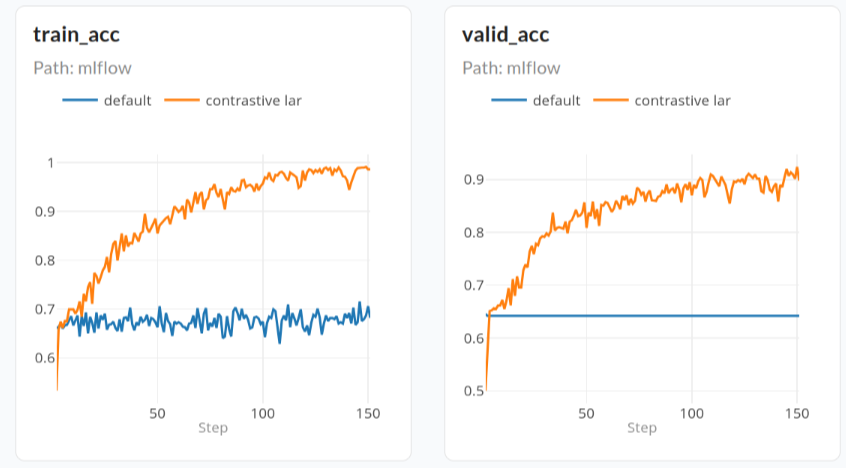
\includegraphics[width=.4\textwidth]{img/accuracy.png}
	\hspace{4em}
	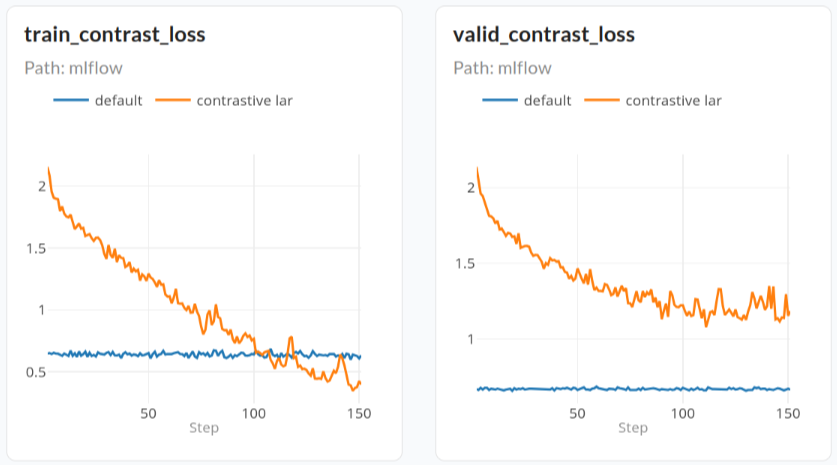
\includegraphics[width=.4\textwidth]{img/loss.png}
	\caption{Plots comparing benchmark cross-entropy loss, training and validation accuracy. The web version of this comparison can be found \href{https://dagshub.com/jinensetpal/contrastive-optimization/experiments\#/compare?experiments=[\%22m_f4f7dea52fa74739be788e5f47da1195\%22,\%22m_1301bf1ba9bf4db48e09e7497c8cd214\%22]}{here}. The blue line represents cross-entropy loss, while the orange line represents the contrastive approach.}
\end{figure}

Crucially, on comparing contrastive activation maps, we can see that each of the cases of the random sample, the model uses the target region for prediction and not spurious features. In the case of the standard training procedure, this is not the case, and the model does not focus on the target in making it's prediction.

\begin{figure}[H]
	\centering
	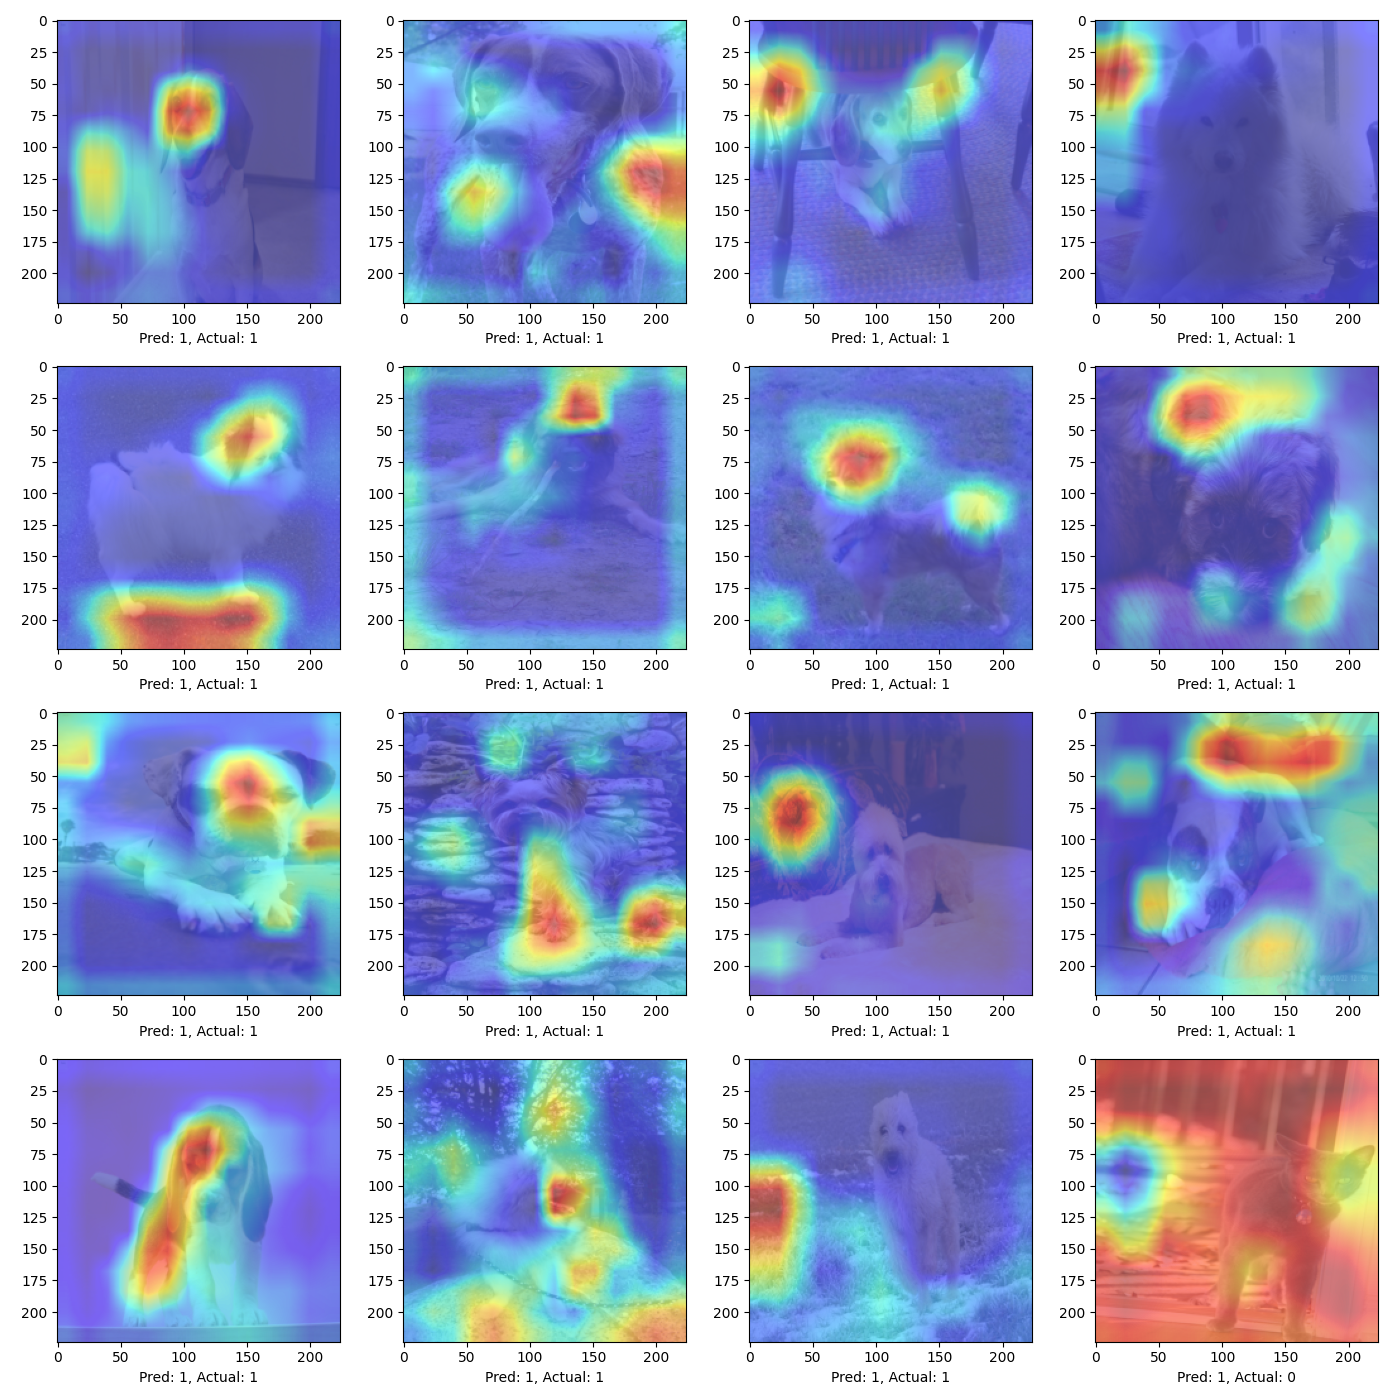
\includegraphics[width=.4\textwidth]{img/default_cam.png}
	\hspace{3em}
	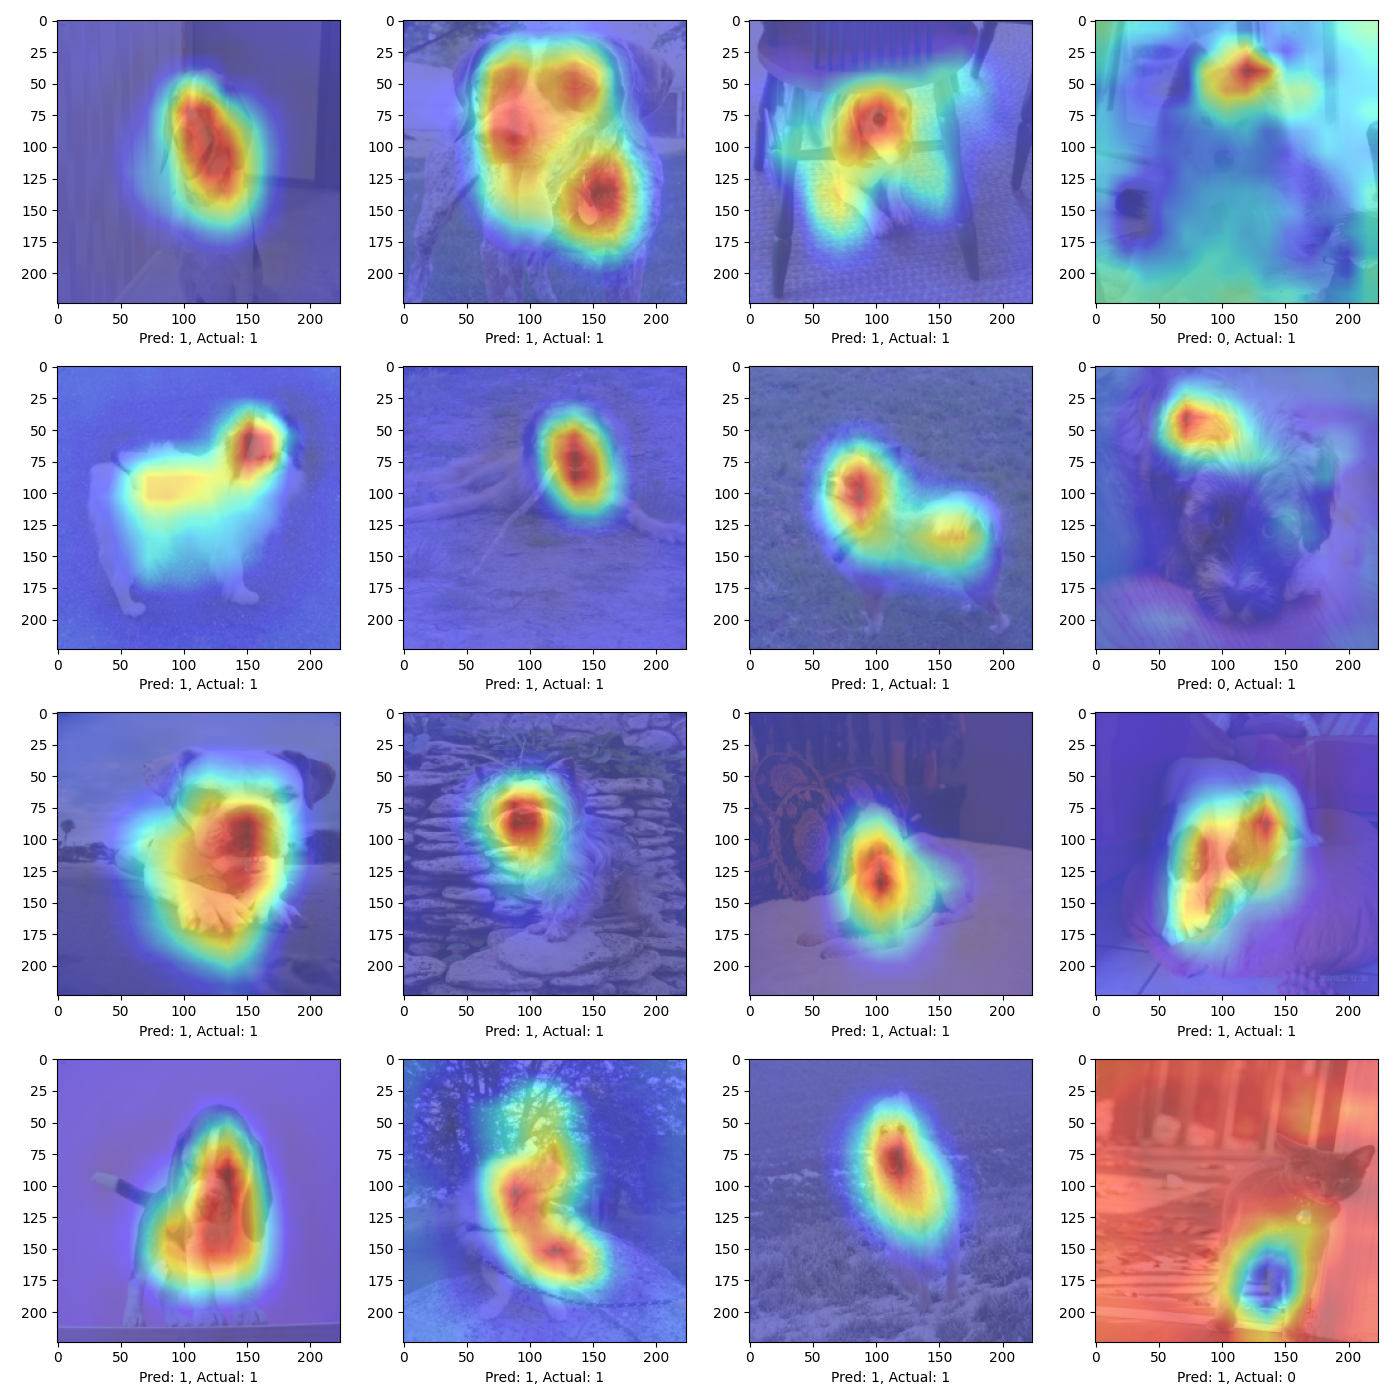
\includegraphics[width=.4\textwidth]{img/contrastive_cam.png}
	\caption{Left: contrastive activation maps from the default training run. Right: contrastive activation maps from the contrastive training run.}
\end{figure}

\subsection{Multiclass Classification}

For multiclass classification, the objective is to distinguish between the features of species within the cat and dog families. There are a total of 37 classes, with a success of rate of $\approx 2.7\%$ with random guessing. There is virtually no class imbalance in this case.

Our approach's performance on the Oxford-IIIT Pets Dataset to the default is as follows:

\begin{table}[h]
	\centering
	\begin{tabular}{c|ccc}
		\toprule
		\textbf{Method}  & \textbf{Cross Entropy Loss}  & \textbf{Training Accuracy}   & \textbf{Validation Accuracy} \\
		\midrule
		Cross-Entropy & 3.627 & 2.8\% & 3.1\% \\
		Interpretable (Ours) & \bf 2.743 & \bf 93.0\% & \bf 51.5\% \\
		\bottomrule
	\end{tabular}
\end{table}

We can observe that the default model is unable to learn any valuable information, the contrastive model is able to learn a significant portion of the information, although with a substantial generalization gap.

The model was trained for 731 epochs with the Adam optimizer with a learning rate of $10^{-3}$ with a batch size of 12, with 5 gradient accumulation steps (effective batch size of 60) on a 32GB V100 on a randomly shuffled dataset using the original splits. The default model was only trained for 30 epochs, by which point it had already converged. For posterity, we will run the default setup for 731 epochs as well before publication.

\subsection{Out-of-Distribution Generalization}

To test how well the approach generalizes out of the training distribution, we evaluate the performance of the binary classification contrastive model on random samples ($n=1000$) from the \href{https://www.microsoft.com/en-us/download/details.aspx?id=54765}{Kaggle Cats and Dogs Dataset}:
\begin{table}[h]
	\centering
	\begin{tabular}{c|c}
		\toprule
		\textbf{Method} & \textbf{Accuracy} \\
		\midrule
		Cross-Entropy & 49.5\% \\
		Interpretable (Ours) & \bf 78.5\% \\
		\bottomrule
	\end{tabular}
\end{table}

The next goal is to further understand and minimize this generalization gap.

\section{Upcoming / In Progress Tasks} 

\paragraph{Understanding the Generalization Gap} While the model for the multiclass paradigm is able to fit the training dataset excellently -- achieving $\approx 93\%$ training accuracy -- the validation accuracy is significantly behind at $\approx 51\%$. This could imply memorization of samples, which was something that this approach was intended to mitigate. Further investigation could help support or disprove this hypothesis.

\paragraph{Evaluating Adversarial Robustness} Could the model looking only at the object to affect the classification score improve adversarial performance?

\paragraph{Mechanistic Interpretability Study} Does the better focus of the model encourage the creation of new image circuits? How does the model perform in cases when it contains neither cat nor dog? Can we make claims about the confidence of the model?

\paragraph{Non-Reduction of Feature Maps} One step of computing HiResCAMs involves summing each attention map to create a single activation map. Could the multiple foci be useful, and something we can further optimize?

\bibliographystyle{plain}
\bibliography{references}

\end{document}
